%%Last date of edition: 1 Juillet 00
%%Who: Stef
%%What: Nouvelle passes

\concept
\chapter{Composons!}\label{chapitrecomposons}

\centerline{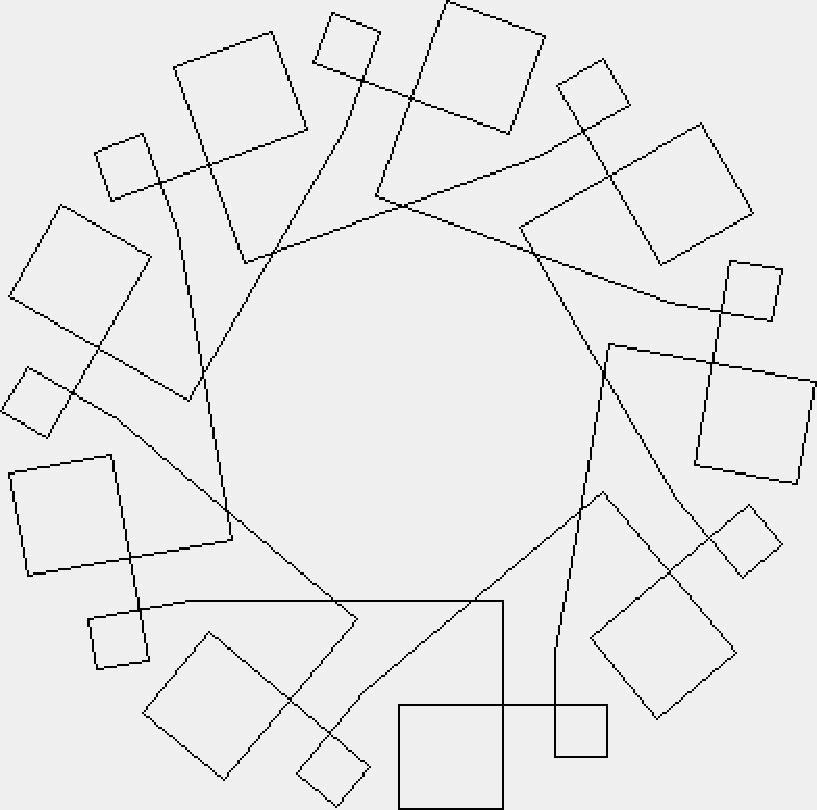
\includegraphics[width=9cm]{c7completething2}}


Lors du pr\'ec\'edent chapitre, nous avons montr\'e comment nous
d\'efinissons de nouvelles m\'ethodes que toutes les tortues
peuvent ex\'ecuter ensuite. Nous avons montr\'e que d\'efinir de
 nouvelles m\'ethodes est int\'eressant car :

\begin{itemize}
\item cela \'evite de devoir r\'e\'ecrire des scripts et 
d'introduire des erreurs, 
\item  et que les m\'ethodes peuvent \^etre utilis\'ees 
par diff\'erentes tortues.
\end{itemize}

L'autre avantage que nous allons explorer dans ce chapitre et dans la
suite du cours est la possibilit\'e de composer des m\'ethodes,
c'est-\`a-dire qu'une m\'ethode est d\'efinie en utilisant d'autres
m\'ethodes. Pouvoir composer des m\'ethodes est extr\^emement
important car cela permet de d\'efinir une m\'ethode en fonction
d'autres m\'ethodes sans avoir \`a conna\^itre comment ces autres
m\'ethodes sont d\'efinies.


\section{Exemple: la m\'ethode \ct{square100}}
Composer des m\'ethodes est assez naturel et n'est pas nouveau. C'est
ce que nous avons fait lors du chapitre pr\'ec\'edent lorsque nous
avons d\'efini des m\'ethodes ! Par exemple, la m\'ethode
\ct{square100} est d\'efinie en faisant appel aux m\'ethodes
\turnLeft, \trace, \noTrace... Elle est donc compos\'ee d'autres messages 
et nous ne faisons pas attention de savoir comment ces messages
\'etaient eux-m\^emes d\'efinis.

\begin{nmethode}
square100
        
   self trace. 
   4 timesRepeat: [self turnLeft:90. 
                  self go: 100].
   self noTrace
\end{nmethode}



\section{Des choses et d'autres: \ct{thing}}
Lors du chapitre~\ref{chapitreenseigner}, vous avez d\'efini la
m\'ethode \ct{thing} qui dessinait la Figure~\ref{c7thing} dont nous
vous rappelons la d\'efinition de la m\'ethode
\ct{thing}. Si vous avez oubli\'e de la sauver vous devez la
red\'efinir \`a l'aide de l'\'editeur.

\begin{figure}[!htbp]
\begin{minipage}[c]{.55\linewidth}
\begin{nmethode}
thing
   "draws a thing"

   self go: 100.
   self turnRight: 90.
   self go: 100.
   self turnRight: 90.
   self go: 50.
   self turnRight: 90.
   self go: 50.
   self turnRight: 90.
   self go: 100.
   self turnRight: 90.
   self go: 25.
   self turnRight: 90.
   self go: 25.
   self turnRight: 90.
   self go: 50
\end{nmethode}
\end{minipage}
\begin{minipage}[c]{.45\linewidth}
\centerline{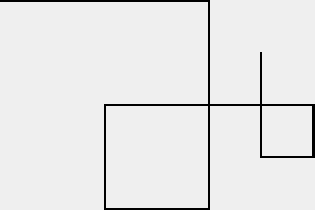
\includegraphics[width=\linewidth]{c6thing}}
\end{minipage}
\caption{\ct{thing} : une dr\^ole de chose.}
\label{c7thing}
\end{figure}

\exercice{Motifs}
\paragraph{\ct{completeThing}.}
D\'efinissez la m\'ethode \ct{completeThing} qui appelle quatre fois
\ct{thing} et r\'ealise la figure compl\`ete  et dont on montre un appel 
 dans la Figure~\ref{c7completething}.


%\begin{figure}[!htbp]
%\centerline{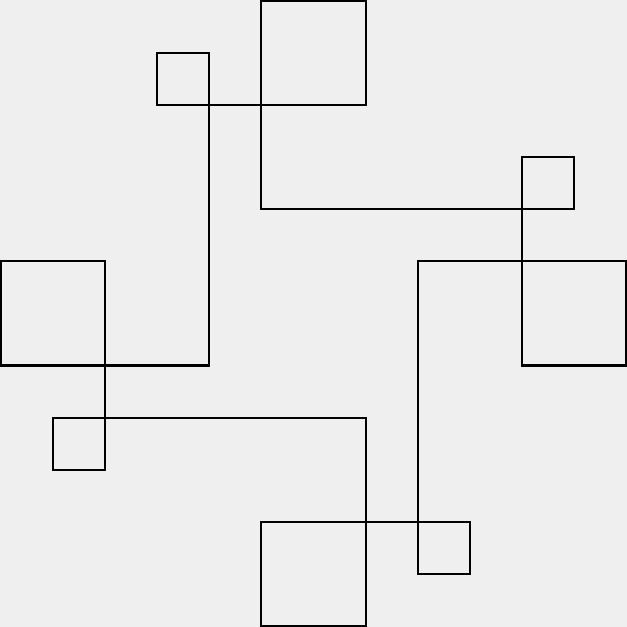
\includegraphics[width=9cm]{c7completething}}
%\caption{Composition de \ct{thing}: \ct{completeThing}.}
%\label{c7completething}
%\end{figure}

\begin{figure} 
\begin{minipage}[t]{.55\linewidth}
\begin{ncscript}{Utilisation de la m\'ethode completeThing}
| caro |
caro := Turtle new.
caro trace.
caro completeThing
\end{ncscript}
\end{minipage}
\begin{minipage}{.45\linewidth}
\centerline{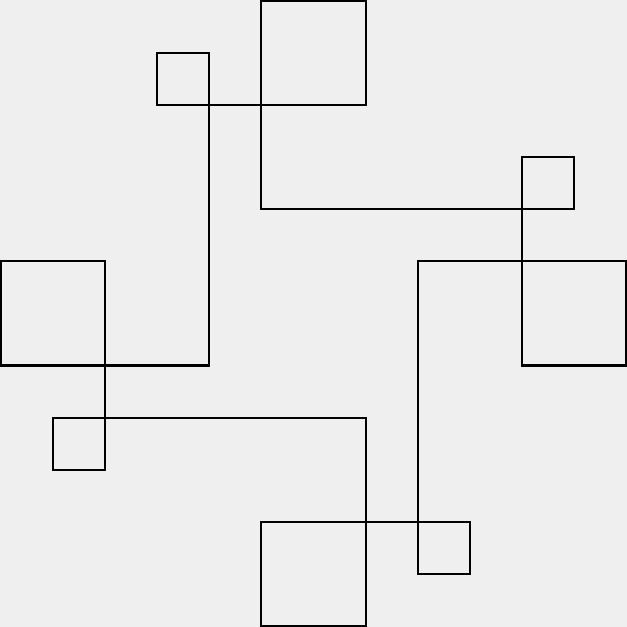
\includegraphics[width=\linewidth]{c7completething}}
\end{minipage}
\caption{\ct{completeThing} : un motif complet.}
\label{c7completething}
\end{figure}


\paragraph{\ct{completeThing2}.} D\'efinissez la m\'ethode \ct{completeThing2} qui dessine la Figure~\ref{c7completething2} et dont on donne la d\'efinition.

\begin{figure} 
\begin{minipage}[c]{.55\linewidth}
\begin{nmethode}
completeThing2 "Draws another complete thing"

   9 timesRepeat: [self thing. 
                  self turnRight: 10. 
                  self go: 50]
\end{nmethode}
\begin{ncscript}{Utilisation de la m\'ethode completeThing2}
| caro |
caro := Turtle new.
caro trace.
caro completeThing2
\end{ncscript}
\end{minipage}
\hfill
\begin{minipage}[c]{.45\linewidth}
\centerline{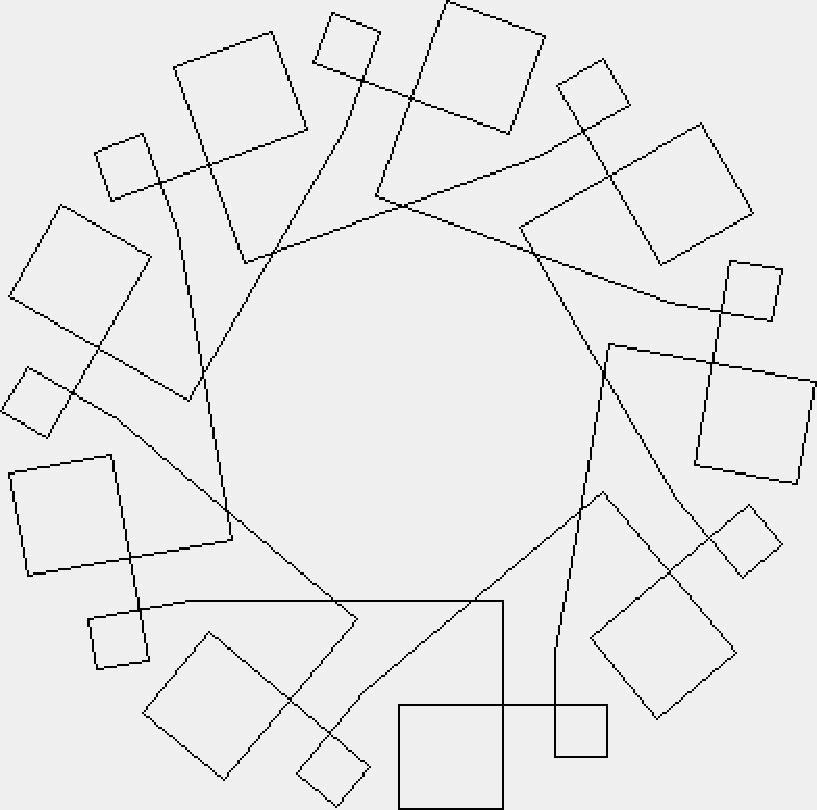
\includegraphics[width=\linewidth]{c7completething2}}
\end{minipage}
\caption{\ct{completeThing2} : un autre motif complet.}
\label{c7completething2}
\end{figure}

%\begin{figure}[!htbp]
%\centerline{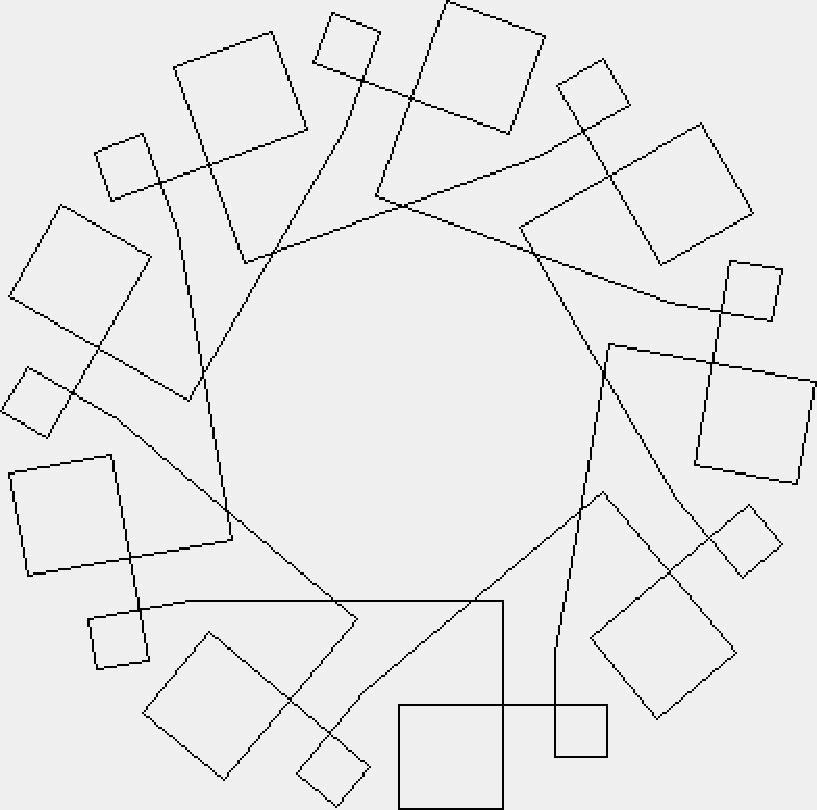
\includegraphics[width=9cm]{c7completething2}}
%\caption{Une autre r\'eutilisation de \ct{thing} : \ct{completeThing2}.}
%\label{c7complete2}
%\end{figure}


\paragraph{\ct{multipleThings}.}
D\'efinissez la m\'ethode \ct{multipleThings} qui dessine la Figure~\ref{c7multipleThings}.

\begin{figure} 
\begin{minipage}[c]{.55\linewidth}
\begin{nmethode}
multipleThings
    "Draws another thing based picture"

    8 timesRepeat: [self thing. 
                   self turnLeft: 45. 
                   self go: 100]
\end{nmethode}
\begin{ncscript}{Utilisation de la m\'ethode \ct{multipleThings}}
| caro |
caro := Turtle new.
caro trace.
caro multipleThings
\end{ncscript}
\end{minipage}
\hfill
\begin{minipage}[c]{.45\linewidth}
\centerline{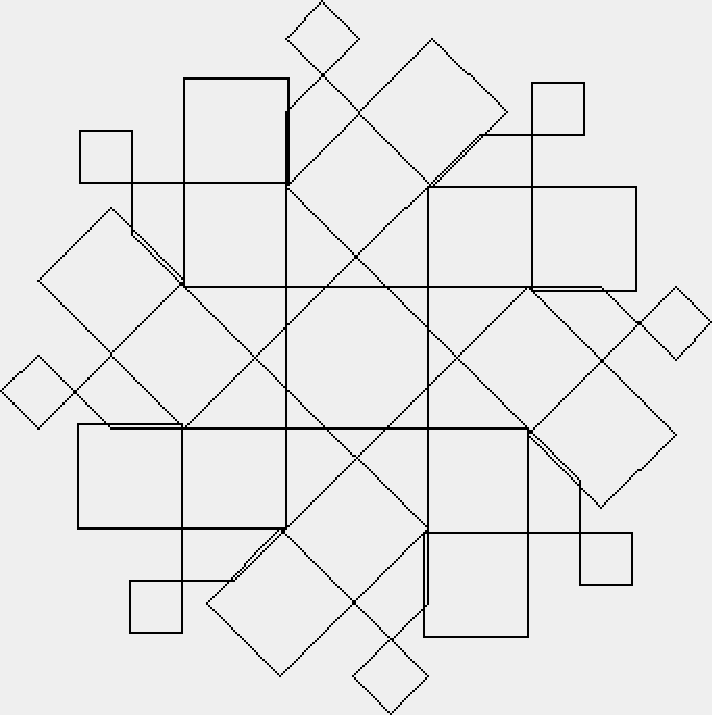
\includegraphics[width=\linewidth]{c7things}}
\end{minipage}
\caption{\ct{multipleThings} : un autre motif encore plus fou.}
\label{c7multipleThings}
\end{figure}



\subsection{Qu'avons-nous mis en \'evidence ? la r\'eutilisation!}
Comme vous le voyez avec les m\'ethodes \ct{completeThing},
\ct{completeThing2} et \ct{multipleThings}, la m\'ethode \ct{thing}
n'est d\'efinie qu'une seule fois, mais est r\'eutilis\'ee plusieurs
fois par les m\'ethodes \ct{completeThing}, \ct{completeThing2} et
\ct{multipleThings} pour produire des dessins diff\'erents. 
La d\'efinition de \ct{thing} comme une m\'ethode nous a donc permis
de~: (1) la d\'efinir une seule fois, (2) r\'eutiliser cette m\'ethode
dans diff\'erents contextes et (3) de ne pas introduire d'erreurs lors
des red\'efinitions.

\subsection{Qu'avons-nous mis en \'evidence ? l'abstraction}
Si vous regardez attentivement la d\'efinition de la m\'ethode
\ct{multipleThings}, vous constatez qu'elle est d\'efinie en termes de la 
m\'ethode \ct{thing} qui elle est aussi d\'efinie en termes d'autres
m\'ethodes comme \go, \turnLeft...

\begin{nmethode}
multipleThings
   "Draws another thing based picture"

   8 timesRepeat: [self thing. 
                  self turnLeft: 45. 
                  self go: 100]
\end{nmethode}

En fait, une m\'ethode plus complexe est souvent d\'efinie en faisant
appel \`a des m\'ethodes plus simples et ainsi de suite. 
Il est essentiel de comprendre que lorsque l'on d\'efinit la m\'ethode
\ct{multipleThings} nous ne voulons pas savoir comment la m\'ethode
\ct{thing} est d\'efinie, nous voulons juste l'utiliser ! 
De cette fa\c con, il est plus simple pour nous de d\'efinir des
m\'ethodes en fonction d'autres sans avoir \`a retenir leur propre
d\'efinition. Nous avons juste \`a nous rappeler ce qu'elles font et
non comment elles le font. On dit que nous nous abstrayons de leur
d\'efinition, c'est pourquoi on dit aussi qu'une m\'ethode d\'efinit
une abstraction.

Pour bien vous montrer cela nous avons r\'eecrit la m\'ethode
\ct{multipleThings} sans appel \`a la m\'ethode \ct{thing}. 
Au lieu de cela nous avons recopi\'e directement la d\'efinition de
\ct{thing} (en italique) \`a l'int\'erieur de \ct{multipleThings}.

\begin{nmethode}
multipleThingsSansUtiliserThing 
   "Draws another thing based picture"

   8 timesRepeat: [\strong{self go: 100.
                  self turnRight: 90.
                  self go: 100.
                  self turnRight: 90.
                  self go: 50.
                  self turnRight: 90.
                  self go: 50.
                  self turnRight: 90.
                  self go: 100.
                  self turnRight: 90.
                  self go: 25.
                  self turnRight: 90.
                  self go: 25.
                  self turnRight: 90.
                  self go: 50thing.}
                  self turnLeft: 45. 
                  self go: 100]
\end{nmethode}

Comparer la m\'ethode \ct{multipleThings} et \ct{thingsSansUtiliserThing}. 
\ct{multipleThings} appara\^it comme bien plus simple. Imaginez maintenant 
ce que pourrait \^etre la m\'ethode \ct{thingsSansUtiliserThing} si
l'on montrait le code des m\'ethodes \go, \turnLeft et \turnRight.

\important{On peut d\'efinir une m\'ethode en fonction d'autres 
m\'ethodes et ceci sur plusieurs niveaux sans avoir \`a comprendre 
comment ces m\'ethodes ont elles-m\^emes \'et\'e construites.}



\section{Des carr\'es partout}
Vous allez maintenant cr\'eer des figures nouvelles \`a l'aide de la
m\'ethode \ct{square100}.


\subsection{Carr\'es et variations}

\exercice{Un gros carr\'e.}
D\'efinissez les m\'ethodes \ct{box} et \ct{separatedBox} qui produisent les dessins de la Figure~\ref{c7groscarre}.

\begin{figure}[!htbp]
\begin{minipage}[c]{.4\linewidth}
\centerline{
\includegraphics[width=\linewidth]{c7groscarre}}
\end{minipage}
\hfill
\begin{minipage}[c]{.4\linewidth}
\centerline{
\includegraphics[width=\linewidth]{c7groscarre2}}
\end{minipage}
\caption{Un carr\'e et un autre.}
\label{c7groscarre}
\end{figure}
 

% solution exercice
%\begin{ncscript}{Un gros carr\'e}
%| caro |
%caro := Turtle new.
%4 timesRepeat: [caro square100.
%               caro turnLeft: 90]
%\end{ncscript}

\exercice{Variantes} Changez le script ci-dessus pour obtenir diff\'erentes 
figures. Vous pouvez changer l'angle, faire avancer la tortue d'une
certaine longueur....Essayer de reproduire la Figure~\ref{c7star}.

%\begin{figure}[!htbp]
%\centerline{
\includegraphics[width=7.5cm]{c7groscarre2}}
%\caption{Variations autour d'un carr\'e.}
%\label{c7groscarre2}
%\end{figure}


%solution variation
%\begin{ncscript}{Une variation}
%| caro |
%caro := Turtle new.
%12 timesRepeat: [caro square100.
%                caro turnLeft: 30.
%                caro go: 10]
%\end{ncscript}


\exercice{\ct{star}.} En utilisant la m\'ethode \ct{box}, 
exp\'erimentez et d\'efinissez le script qui produit l'\'etoile
Figure~\ref{c7star}.


\begin{figure}[!htbp]
\begin{minipage}[c]{.4\linewidth}
\centerline{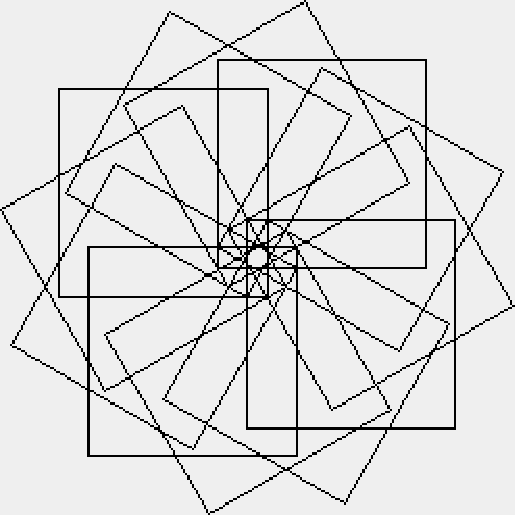
\includegraphics[width=7cm]{c7carrevar1}}
\end{minipage}
\hfill
\begin{minipage}[c]{.4\linewidth}
\centerline{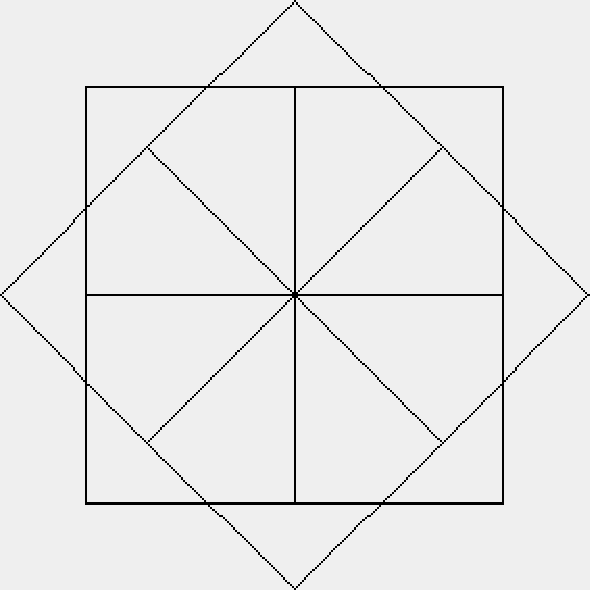
\includegraphics[width=7cm]{c7star}}
\end{minipage}
\caption{Variations autour d'un carr\'e et une \'etoile.}
\label{c7star}
\end{figure}

